% !TEX root = ../presentation.tex
% Deep Learning

\begin{slide}{Deep Neural Networks}
  \only<2>{
    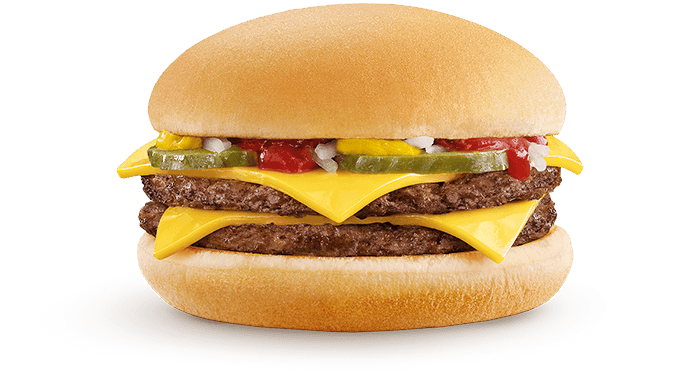
\includegraphics[scale=0.25]{burger}
  }
  \only<3>{
  \begin{tikzpicture}
    % Pixels
      \foreach \x in {0, 0.25, ..., 3.75} {
        \foreach \y in {0, 0.25, ..., 3.75} {
          \randomcolor
          \fill [randomcolor] (\x, \y) rectangle ++(0.25, 0.25);
        }
      }
  \end{tikzpicture}
  }
  \only<4>{
  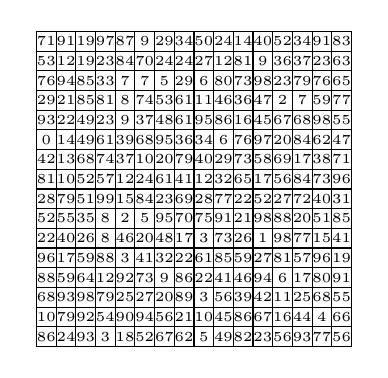
\begin{tikzpicture}
    % Pixels
      \foreach \x in {0, 0.25, ..., 3.75} {
        \foreach \y in {0, 0.25, ..., 3.75} {
          \draw (\x, \y) rectangle ++(0.25, 0.25) node [midway] {\tiny\pdfuniformdeviate 100};
        }
      }
  \end{tikzpicture}
  }
  \only<5->{
  \begin{tikzpicture}
    % R layer (feature map)
    % \onslide<8->{
    % \yzplane{0}{
    %   \fill [ProcessBlue] (0, 0) rectangle ++(4, 4);
    % }
    % \xyplane{0}{
    %   \fill [ProcessBlue] (0, 0) rectangle ++(0.3, 4);
    % }
    % \xyplane{4}{
    %   \fill [ProcessBlue] (0, 0) rectangle ++(0.3, 4);
    % }
    % \xzplane{0}{
    %   \fill [ProcessBlue] (0, 0) rectangle ++(0.3, 4);
    % }
    % \xzplane{4}{
    %   \fill [ProcessBlue] (0, 0) rectangle ++(0.3, 4);
    % }
    % }

    % G layer (feature map)
    % \onslide<7->{
    % \yzplane{0.6}{
    %   \fill [Green] (0, 0) rectangle ++(4, 4);
    % }
    % \yzplane{0.9}{
    %   \fill [Green] (0, 0) rectangle ++(4, 4);
    % }
    % \xyplane{0}{
    %   \fill [Green] (0.6, 0) rectangle ++(0.3, 4);
    % }
    % \xyplane{4}{
    %   \fill [Green] (0.6, 0) rectangle ++(0.3, 4);
    % }
    % \xzplane{0}{
    %   \fill [Green] (0.6, 0) rectangle ++(0.3, 4);
    % }
    % \xzplane{4}{
    %   \fill [Green] (0.6, 0) rectangle ++(0.3, 4);
    % }
    % }

    % B layer (feature map)
    % \onslide<6->{
    % \yzplane{1.2}{
    %   \fill [Red] (0, 0) rectangle ++(4, 4);
    % }
    % \yzplane{1.5}{
    %   \fill [Red] (0, 0) rectangle ++(4, 4);
    % }
    % \xyplane{0}{
    %   \fill [Red] (1.2, 0) rectangle ++(0.3, 4);
    % }
    % \xyplane{4}{
    %   \fill [Red] (1.2, 0) rectangle ++(0.3, 4);
    % }
    % \xzplane{0}{
    %   \fill [Red] (1.2, 0) rectangle ++(0.3, 4);
    % }
    % \xzplane{4}{
    %   \fill [Red] (1.2, 0) rectangle ++(0.3, 4);
    % }
    % }

    % Pixels
    \yzplane{1.8}{
      \foreach \y in {0, 0.25, ..., 3.75} {
        \foreach \z in {0, 0.25, ..., 3.75} {
          \randomcolor
          \fill [randomcolor] (\y, \z) rectangle ++(0.25, 0.25);
        }
      }
    }
  \end{tikzpicture}
  }
\end{slide}

\begin{slide}{Deep Neural Networks}
  \begin{itemize}
    \item<1-> We want to classify images into one of $k$ classes
    \item<2-> Extract hierarchical features
    \vspace{1cm}

    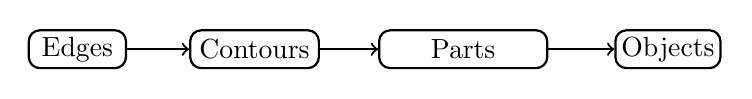
\begin{tikzpicture}[thick]
      \onslide<3->{
      \path (0, 0) coordinate
            [draw, rectangle, rounded corners, text width=1cm, text height = 7pt]
            (e) node {Edges};
      }

      \onslide<4->{
        \path (2.25, 0) coordinate
              [draw, rectangle, rounded corners, text width=1.4cm, text height = 7pt]
              (cont) node {Contours};
        \draw [->] (e) -- (cont);
      }

      \onslide<5->{
        \path (4.9, 0) coordinate
              [draw, rectangle, rounded corners, text width=1.9cm, text height = 7pt]
              (parts) node {Parts};
        \draw [->] (cont) -- (parts);
      }

      \onslide<6->{
        \path (7.5, 0) coordinate
              [draw, rectangle, rounded corners, text width=1.1cm, text height = 7pt]
              (o) node {Objects};
        \draw [->] (parts) -- (o);
      }
    \end{tikzpicture}
  \end{itemize}
\end{slide}

\begin{slide}{Deep Neural Networks}
  \frameheader{Why reinvent the wheel?}

  \begin{tikzpicture}[thick]
    \only<2> {
     % First picture
      \foreach \x in {0, ..., 2} {
        \foreach \y in {0, ..., 2} {
          \draw (\x, \y) rectangle ++(1, 1) node [midway] {\random{100}};
        }
      }
    }

    % Flattened pixels (input layer)
    \only<3-> {
      \foreach \i in {0, ..., 8} {
        \draw (0, {\i/2}) rectangle ++(0.5, 0.5) node [midway] {\random{100}};
      }
    }

    % First hidden layer
    \only<4-> {
      \foreach \i in {0, ..., 3} {
        \path (2, {(3 - \i) + 0.75}) coordinate [draw, circle, inner sep=7pt]
              (h1\i)
              node {$h_\i$};
      }
    }

    % Iteratively draw connections from the input nodes to the first layer
    \newcount\slidecount\relax
    \slidecount=5\relax
    \foreach \x in {0, 0.5, ..., 4} {
      \only<\the\slidecount-> {
        \foreach \i in {0, ..., 3} {
          \draw [->, semithick] (0.5, {\x + 0.25}) -- (h1\i);
        }
      }
      \global\advance\slidecount by 1\relax
    }

    % Second hidden layer
    \only<14-> {
      \foreach \h in {0, ..., 5} {
        \path (4, {5 - \h - 0.25})
              coordinate [draw, circle, inner sep=7pt]
              (h2\h)
              node {$h_\h$};

        \foreach \i in {0, ..., 3} {
          \draw [->, semithick] (h1\i) -- (h2\h);
        }
      }
    }

    % Third hidden layer
    \only<15-> {
      \foreach \h in {0, ..., 5} {
        \path (6, {5 - \h - 0.25})
              coordinate [draw, circle, inner sep=7pt]
              (h3\h)
              node {$h_\h$};

        \foreach \i in {0, ..., 5} {
          \draw [->, semithick] (h2\i) -- (h3\h);
        }
      }
    }

    % Output hidden layer
    \only<16-> {
      \foreach \y in {0, ..., 2} {
        \path (8, {2 - \y + 1.25})
              coordinate [draw, circle, inner sep=7pt]
              (y\y)
              node {$y_\y$};

        \foreach \i in {0, ..., 5} {
          \draw [->, semithick] (h3\i) -- (y\y);
        }
      }
    }

    % Labels
    \only<17-> { \draw (y0)+(1.25, 0) node {unicorn}; }
    \only<18-> { \draw (y1)+(1.2, 0) node {teapot}; }
    \only<19-> { \draw (y2)+(0.95, 0) node {car}; }
  \end{tikzpicture}
\end{slide}

% \begin{slide}{Convolutional Neural Networks}
%   $$
%   \begin{sbmatrix}{R}
%     116 & 80 \\
%     170 & 194 \\
%   \end{sbmatrix}
%   \hspace{0.5cm}
%   \begin{sbmatrix}{G}
%     82 & 78 \\
%     5 & 236 \\
%   \end{sbmatrix}
%   \hspace{0.5cm}
%   \begin{sbmatrix}{B}
%     76 & 139 \\
%     245 & 236 \\
%   \end{sbmatrix}
%   $$
%   \pause
%   \texttt{concatenate(}$R$\texttt{.flatten, }$G$\texttt{.flatten, }$B$\texttt{.flatten}\texttt{)}
% \end{slide}
%
% \begin{slide}{Convolutional Neural Networks}
%   $$
%   \begin{sbmatrix}{R}
%     116 & 80 \\
%     170 & 194 \\
%   \end{sbmatrix}
%   \hspace{0.5cm}
%   \begin{sbmatrix}{G}
%     82 & 78 \\
%     5 & 236 \\
%   \end{sbmatrix}
%   \hspace{0.5cm}
%   \begin{sbmatrix}{B}
%     76 & 139 \\
%     245 & 236 \\
%   \end{sbmatrix}
%   $$
%   \begin{align*}
%     R\mathtt{.flatten} &= \begin{bmatrix}116 & 80 & 170 & 194\end{bmatrix}
%   \end{align*}
% \end{slide}
%
% \begin{slide}{Convolutional Neural Networks}
%   $$
%   \begin{sbmatrix}{R}
%     116 & 80 \\
%     170 & 194 \\
%   \end{sbmatrix}
%   \hspace{0.5cm}
%   \begin{sbmatrix}{G}
%     82 & 78 \\
%     5 & 236 \\
%   \end{sbmatrix}
%   \hspace{0.5cm}
%   \begin{sbmatrix}{B}
%     76 & 139 \\
%     245 & 236 \\
%   \end{sbmatrix}
%   $$
%   \begin{align*}
%     R\mathtt{.flatten} &= \begin{bmatrix}116 & 80 & 170 & 194\end{bmatrix}\\
%     G\mathtt{.flatten} &= \begin{bmatrix}82 & 78 & 5 & 236\end{bmatrix}
%   \end{align*}
% \end{slide}
%
% \begin{slide}{Convolutional Neural Networks}
%   $$
%   \begin{sbmatrix}{R}
%     116 & 80 \\
%     170 & 194 \\
%   \end{sbmatrix}
%   \hspace{0.5cm}
%   \begin{sbmatrix}{G}
%     82 & 78 \\
%     5 & 236 \\
%   \end{sbmatrix}
%   \hspace{0.5cm}
%   \begin{sbmatrix}{B}
%     76 & 139 \\
%     245 & 236 \\
%   \end{sbmatrix}
%   $$
%   \begin{align*}
%     R\mathtt{.flatten} &= \begin{bmatrix}116 & 80 & 170 & 194\end{bmatrix}\\
%     G\mathtt{.flatten} &= \begin{bmatrix}82 & 78 & 5 & 236\end{bmatrix}\\
%     B\mathtt{.flatten} &= \begin{bmatrix}76 & 139 & 245 & 236\end{bmatrix}
%   \end{align*}
% \end{slide}
%
% \begin{slide}{Convolutional Neural Networks}
%   $$
%   \begin{sbmatrix}{R}
%     116 & 80 \\
%     170 & 194 \\
%   \end{sbmatrix}
%   \hspace{0.5cm}
%   \begin{sbmatrix}{G}
%     82 & 78 \\
%     5 & 236 \\
%   \end{sbmatrix}
%   \hspace{0.5cm}
%   \begin{sbmatrix}{B}
%     76 & 139 \\
%     245 & 236 \\
%   \end{sbmatrix}
%   $$
%
%   \begin{align*}
%     R\mathtt{.flatten} &= \begin{bmatrix}116 & 80 & 170 & 194\end{bmatrix}\\
%     G\mathtt{.flatten} &= \begin{bmatrix}82 & 78 & 5 & 236\end{bmatrix}\\
%     B\mathtt{.flatten} &= \begin{bmatrix}76 & 139 & 245 & 236\end{bmatrix}
%   \end{align*}
%
%   $$\mathbf{x} = \begin{bmatrix}116,  80, 170, 194,  82,  78,   5, 236,  76, 139, 245, 236\end{bmatrix}$$
% \end{slide}
%
% \begin{slide}{Convolutional Neural Networks}
%   \frameheader{Why is this a bad idea?}
%   \begin{enumerate}
%     \pitem Fully connected NNs scale badly for images
%     \begin{itemize}
%       \pitem $200 \times 200 \times 3 = 120,000$ features
%       \pitem With 100 hidden units: $100 \times 120,000 = 12,000,000$
%       % \pitem With 5 layers: $12,000,000 \times 5 = 60,000,000$ weights
%       % \pitem $1000 \times 1000 \rightarrow 1,500,000,000$ weights
%     \end{itemize}
%     \pitem It assumes every pixel has entirely new information
%   \end{enumerate}
% \end{slide}

\begin{slide}{Convolutional Neural Networks}
  \only<1>{

    % trim = {left bottom right above}
    
\includegraphics[scale=0.25, trim={0 0 0 4cm}, clip]{cat}

    \vspace{0.2cm}

    This is a cat $\varheart$
  }
  \only<2>{
    \includegraphics[scale=0.2]{cat2}

    \vspace{0.2cm}

    Still a cat $\varheart\varheart$
  }
  \only<3>{
    \includegraphics[scale=0.3]{cat4}

    \vspace{0.2cm}

    Half cat / half salad $\varheart\varheart\varheart$
  }
  \only<4>{
    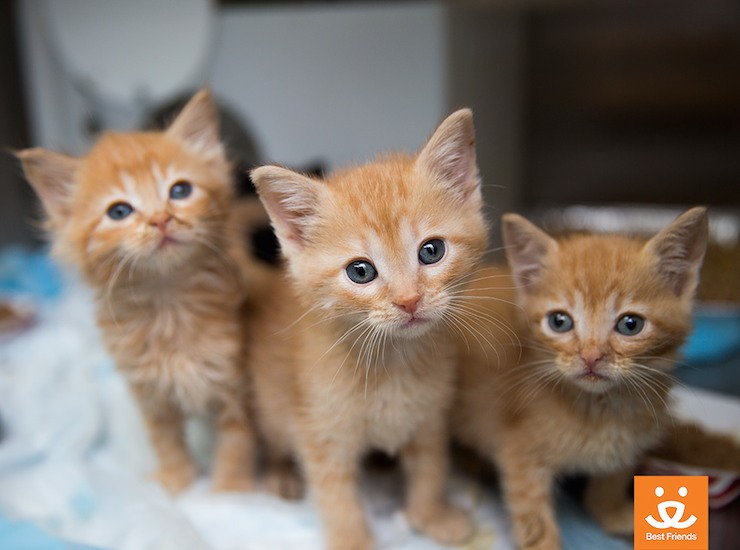
\includegraphics[scale=0.3, trim={0 3cm 0 0cm}, clip]{cats}

    \vspace{0.2cm}

    Many cats $\varheart\varheart\varheart\varheart$
  }
\end{slide}

% If the network learns to recognize a feature in one layer
% Wouldn't it make sense to reuse that information elsewhere

\begin{slide}{Convolutional Neural Networks}
  {
    \Huge
    Weight Sharing
  }
\end{slide}

\begin{slide}{Convolutional Neural Networks: Mechanics}
  \frameheader{Weight Sharing}

  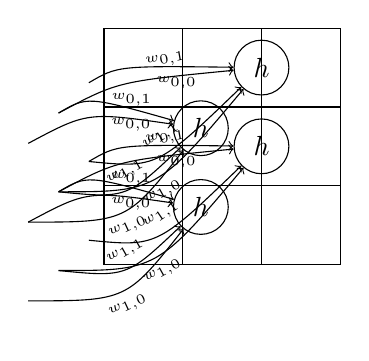
\begin{tikzpicture}
    \yzplane{0}{
      \foreach \y in {0, ..., 2} {
        \foreach \z in {0, ..., 2} {
          % \randomcolor
          % \fill [randomcolor] (\y, \z) rectangle ++(1, 1);
          \draw (\y, \z) rectangle ++(1, 1);
        }
      }
    }

    \newcount\slidecount\relax
    \slidecount=2\relax
    \foreach \i in {0, 1} {
      \foreach \j in {0, 1} {
        \only<\the\slidecount> {
          \path (2, {2.5-\i}, {2-\j*2})
                coordinate [draw, circle, inner sep=7pt]
                (h\j\i) node {$h$};

          \draw [->] (0, {2.5-\i}, {2.5-\j})
             .. controls (0.75, {2.9-\i}, {2.5-\j}) .. (h\j\i)
             node [pos=0.6, above right, sloped] {\tiny$w_{0,1}$};

          \draw [->] (0, {2.5-\i}, {1.5-\j})
             .. controls (0.75, {3.1-\i}, {2.5-\j}) .. (h\j\i)
             node [pos=0.8, below] {\tiny$w_{0,0}$};

          \draw [->] (0, {1.5-\i}, {2.5-\j})
            .. controls (1.25, {1.5-\i}, {2.5-\j}) .. (h\j\i)
             node [pos=0.5, below, sloped] {\tiny$w_{1,0}$};

          \draw [->] (0, {1.5-\i}, {1.5-\j})
            .. controls (1.25, {1.8-\i}, {2.5-\j}) .. (h\j\i)
             node [pos=0.6, above, sloped] {\tiny$w_{1,1}$};
        }
        \global\advance\slidecount by 1\relax
      }
    }

  \end{tikzpicture}
  % Most importantly, we'd most often have many kernels for each layer
  % So if the input layer has k feature maps, the output layer will have x feature maps
\end{slide}

% \begin{slide}{Digression: Convolutions}
%   \begin{itemize}
%     \item<1-> Convolution is a mathematical operation
%     \item<2-> Used a lot in signal processing
%   \end{itemize}
%
%   \onslide<3->{
%     \begin{tikzpicture}
%       % x axis
%       \draw [->] (0, 0) -- (8.5, 0) node [below left] {$t$};
%
%       % y axis
%       \draw [->] (0, 0) -- (0, 2.5) node [below left] {$s(t)$};
%
%       % x Ticks
%       \foreach \i in {0, 1, ..., 7} {
%         \draw ({\i+0.5}, -0.1) node [below] {$\i$} -- ({\i+0.5}, 0);
%       }
%
%       % y Ticks
%       \foreach \i in {0, 1} {
%         \draw (-0.1, {\i+0.5}) node [left] {$\i$} -- (+0.1, {\i+0.5});
%       }
%
%       % Signal
%       \foreach \x in {0.5, 1, ..., 8} {
%         \draw [ProcessBlue] (\x, 0) -- (\x, {((rand+1)/2)*1.5});
%       }
%     \end{tikzpicture}
%   }
%   \onslide<4->{
%   \begin{tikzpicture}
%     % x axis
%     \draw [->] (0, 0) -- (2.3, 0) node [below left] {$t$};
%
%     % y axis
%     \draw [->] (0, 0) -- (0, 2.5) node [below left] {$k(t)$};
%
%     % x Ticks
%     \foreach \i in {0, 1, ..., 1.5} {
%       \draw ({\i+0.5}, -0.1) node [below] {$\i$} -- ({\i+0.5}, 0);
%     }
%
%     % y Ticks
%     \foreach \i in {0, 1} {
%       \draw (-0.1, {\i+0.5}) node [left] {$\i$} -- (+0.1, {\i+0.5});
%     }
%
%     % Signal
%     \foreach \x in {0.5, 1, ..., 1.5} {
%       \draw [Red] (\x, 0) -- (\x, {2-\x});
%     }
%   \end{tikzpicture}
%   }
% \end{slide}

\begin{slide}{Convolutional Neural Networks: Mechanics}
  \begin{tikzpicture}
    % Image
    \draw (0, 0) grid ++(3, 3);

    % Grayscale pixel values
    \only<1>{
      \foreach \x in {0, ..., 2} {
        \foreach \y in {0, ..., 2} {
          \randomgray
          \fill [randomgray] (\x, \y) rectangle ++(1, 1);
        }
      }
    }

    \only<2-3>{
    \draw (0.5, 0.5) node {$0.8$};
    \draw (1.5, 0.5) node {$0.3$};
    \draw (2.5, 0.5) node {$0.5$};
    \draw (0.5, 1.5) node {$0.7$};
    \draw (1.5, 1.5) node {$0.2$};
    \draw (2.5, 1.5) node {$0.6$};
    \draw (0.5, 2.5) node {$0.4$};
    \draw (1.5, 2.5) node {$0.9$};
    \draw (2.5, 2.5) node {$0.1$};
    }

    \draw (1.5, -0.5) node {Image};

    \only<3-3>{
    \draw (4, 0) grid ++(2, 2);

    \draw (4.5, 0.5) node {$3.1$};
    \draw (5.5, 0.5) node {$0.9$};
    \draw (4.5, 1.5) node {$5.7$};
    \draw (5.5, 1.5) node {$2.4$};

    \draw (5, -0.5) node {Kernel};
    }

    \only<4-5>{
      \draw (0.5, 0.5) node {$0.8$};
      \draw (1.5, 0.5) node {$0.3$};
      \draw (2.5, 0.5) node {$0.5$};
      \draw (0.5, 1.5) node {\tiny$3.1 \cdot 0.7$};
      \draw (1.5, 1.5) node {\tiny$0.9 \cdot 0.2$};
      \draw (2.5, 1.5) node {$0.6$};
      \draw (0.5, 2.5) node {\tiny$5.7 \cdot 0.4$};
      \draw (1.5, 2.5) node {\tiny$2.4 \cdot 0.9$};
      \draw (2.5, 2.5) node {$0.1$};

      \draw [red] (0, 1) grid (2, 3);
    }
    \only<5-> {
      \draw [red] (4, 1) rectangle ++(1, 1) node [midway, black] {$6.79$};
      \draw (5, -0.5) node {Output};
    }
    \only<6-7>{
    \draw (0.5, 0.5) node {$0.8$};
    \draw (1.5, 0.5) node {$0.3$};
    \draw (2.5, 0.5) node {$0.5$};
    \draw (0.5, 1.5) node {$0.7$};
    \draw (1.5, 1.5) node {\tiny$3.1 \cdot 0.2$};
    \draw (2.5, 1.5) node {\tiny$0.9 \cdot 0.6$};
    \draw (0.5, 2.5) node {$0.4$};
    \draw (1.5, 2.5) node {\tiny$5.7 \cdot 0.9$};
    \draw (2.5, 2.5) node {\tiny$2.4 \cdot 0.1$};

      \draw [ProcessBlue] (1, 1) grid (3, 3);
    }
    \only<7-> {
      \draw [ProcessBlue] (5, 1) rectangle ++(1, 1) node [black, midway] {$6.53$};
    }
    \only<8-9>{
    \draw (0.5, 0.5) node {\tiny$3.1 \cdot 0.8$};
    \draw (1.5, 0.5) node {\tiny$0.9 \cdot 0.3$};
    \draw (2.5, 0.5) node {$0.5$};
    \draw (0.5, 1.5) node {\tiny$5.7 \cdot 0.7$};
    \draw (1.5, 1.5) node {\tiny$2.4 \cdot 0.2$};
    \draw (2.5, 1.5) node {$0.6$};
    \draw (0.5, 2.5) node {$0.4$};
    \draw (1.5, 2.5) node {$0.9$};
    \draw (2.5, 2.5) node {$0.1$};

      \draw [LimeGreen] (0, 0) grid (2, 2);
    }
    \only<9-> {
      \draw [LimeGreen] (4, 0) rectangle ++(1, 1) node [black, midway] {$7.67$};
    }
    \only<10-11>{
    \draw (0.5, 0.5) node {$0.8$};
    \draw (1.5, 0.5) node {\tiny$3.1 \cdot 0.3$};
    \draw (2.5, 0.5) node {\tiny$0.9 \cdot 0.5$};
    \draw (0.5, 1.5) node {$0.7$};
    \draw (1.5, 1.5) node {\tiny$5.7 \cdot 0.2$};
    \draw (2.5, 1.5) node {\tiny$2.4 \cdot 0.6$};
    \draw (0.5, 2.5) node {$0.4$};
    \draw (1.5, 2.5) node {$0.9$};
    \draw (2.5, 2.5) node {$0.1$};

      \draw [Magenta] (1, 0) grid (3, 2);
    }
    \only<11-> {
      \draw [Magenta] (5, 0) rectangle ++(1, 1) node [black, midway] {$3.96$};
    }
  \end{tikzpicture}
\end{slide}

Required below
\newcommand{\kernel}[1]{
  \xyplane{#1}{
    \draw (0, 2.79) grid [step=0.4] ++(1.2, 1.21);
  }
  \xyplane{{#1+1.2}}{
    \draw (0, 2.79) grid [step=0.4] ++(1.2, 1.21);
  }
  \yzplane{0}{
    \draw (2.79, #1) grid [step=0.4] ++(1.21, 1.21);
  }
  \yzplane{1.2}{
    \draw (2.79, #1) grid [step=0.4] ++(1.21, 1.21);
  }
  \xzplane{4}{
    \draw (0, #1) grid [step=0.4] ++(1.21, 1.21);
  }
  \xzplane{2.8}{
    \draw (0, #1) grid [step=0.4] ++(1.21, 1.21);
  }
}

\begin{slide}{Convolutional Neural Networks: Mechanics}
  \begin{tikzpicture}
    % R layer (feature map)
    \yzplane{0}{
      \draw [ProcessBlue] (0, 0) rectangle ++(4, 4);
    }
    \xyplane{4}{
      \draw [ProcessBlue] (0, 0) rectangle ++(0.4, 4);
    }
    \xzplane{0}{
      \draw [ProcessBlue] (0, 0) rectangle ++(0.4, 4);
    }
    \xzplane{4}{
      \draw [ProcessBlue] (0, 0) rectangle ++(0.4, 4);
    }

    % G layer (feature map)
    \yzplane{0.4}{
      \draw [Green] (0, 0) rectangle ++(4, 4);
    }
    \xyplane{0}{
      \draw [Green] (0.4, 0) rectangle ++(0.4, 4);
    }
    \xyplane{4}{
      \draw [Green] (0.4, 0) rectangle ++(0.4, 4);
    }
    \xzplane{0}{
      \draw [Green] (0.4, 0) rectangle ++(0.4, 4);
    }
    \xzplane{4}{
      \draw [Green] (0.4, 0) rectangle ++(0.4, 4);
    }

    % B layer (feature map)
    \yzplane{0.8}{
      \draw [red] (0, 0) rectangle ++(4, 4);
    }
    \xyplane{0}{
      \draw [red] (0.8, 0) rectangle ++(0.4, 4);
    }
    \xyplane{4}{
      \draw [red] (0.8, 0) rectangle ++(0.4, 4);
    }
    \xzplane{0}{
      \draw [red] (0.8, 0) rectangle ++(0.4, 4);
    }
    \xzplane{4}{
      \draw [red] (0.8, 0) rectangle ++(0.4, 4);
    }

    \newcount\slidecount\relax
    \slidecount=1\relax
    \foreach \i in {0, 0, 0.4, 0.8, 1.2, 1.6, 2, 2.4, 2.8} {

      % Output
      \ifnum\slidecount>1
          \only<\slidecount-9> { \cube{4}{3.2}{\i + 0.4}{0.4} }
      \fi

      % Sliding kernel
      \ifnum\slidecount=9
        \only<\slidecount->{ \kernel{\i} }
      \else
        \only<\slidecount>{ \kernel{\i} }
      \fi

      \global\advance\slidecount by 1\relax
    }

    \foreach \x/\i in {4/10, 4.4/11, 4.8/12} {
      \only<\i-> {
        \yzplane{\x}{
          \draw (0.4, 0.4) rectangle ++(3.2, 3.2);
        }
        \xyplane{0.4}{
          \draw (\x, 0.4) rectangle ++(0.4, 3.2);
        }
        \xyplane{3.6}{
          \draw (\x, 0.4) rectangle ++(0.4, 3.2);
        }
        \xzplane{0.4}{
          \draw (\x, 0.4) rectangle ++(0.4, 3.2);
        }
        \xzplane{3.6}{
          \draw (\x, 0.4) rectangle ++(0.4, 3.2);
        }
      }
    }

  \end{tikzpicture}
\end{slide}

\begin{slide}{Convolutional Neural Networks: Mechanics}
  \frameheader{Recipe for a Convolutional Neural Network Layer}
  \begin{itemize}
    \item<2-> Ingredients
    \begin{enumerate}
      \item<3-> Image $I$ with dimension $w \times h \times d$
      \item<4-> A kernel (filter) $K$ of size $k \times l \times m$
    \end{enumerate}
    \item<5-> Cooking
    \begin{itemize}
      \item<6-> \only<6>{Put the image into the oven at 150\degree C}\only<7->{Don't put the image into the oven at 150\degree C}
      \item<8-> Slide the kernel across the image
      \item<9-> Compute the ``dot product'' for each configuration
      % \item<10-> (This is a convolution $I \ast K$)
    \end{itemize}
  \end{itemize}
\end{slide}

\begin{slide}{Convolutional Neural Networks: Hyperparameters}
  \begin{itemize}
    \item<1-> Convolutional Neural Networks have three hyperparameters
    \begin{enumerate}
      \item<2-> Kernel size % usually odd for valid padding, 3x3 or 5x5
      \item<3-> Kernel stride % usually 1 or 2
      \item<4-> Padding (valid or same)
      % Valid we don't go past th edge, so the spatial dimension will reduce
      % Same padding we do go past the edge and pad the image with zeros
      % then the spatial dimension will stay the same (most common)
    \end{enumerate}
  \end{itemize}
  \vspace{1cm}

  \onslide<4->{
    \begin{tikzpicture}
      \draw (0, 0) grid [step=0.5] (2, 2);
      \foreach \i/\s in {0/5, 0.5/6} {
        \only<\s>{
          \fill [red] (\i, 0.5) rectangle ++(1.5, 1.5);
          \draw (\i, 0.5) grid [step=0.5] ++(1.5, 1.5);
        }
      }
      \newcommand{\drawzeros}{
        \foreach \i in {0, 0.5, ..., 1.5} {
          \draw (\i, -0.5) rectangle ++(0.5, 0.5) node [midway] {0};
          \draw (-0.5, \i) rectangle ++(0.5, 0.5) node [midway] {0};
          \draw (\i, 2) rectangle ++(0.5, 0.5) node [midway] {0};
          \draw (2, \i) rectangle ++(0.5, 0.5) node [midway] {0};
        }
        \foreach \i in {-0.5, 2} {
          \draw (\i, -0.5) rectangle ++(0.5, 0.5) node [midway] {0};
          \draw (\i, 2) rectangle ++(0.5, 0.5) node [midway] {0};
        }
      }
      \only<7-> {
        \drawzeros
      }
      \foreach \i/\s in {-0.5/8, 0/9, 0.5/10, 1/11} {
        \only<\s>{
          \fill [red] (\i, 1) rectangle ++(1.5, 1.5);
          \draw ({\i+0.5}, 1.5) rectangle ++(0.5, 0.5) node [midway] {$\times$};
          \draw (\i, 1) grid [step=0.5] ++(1.5, 1.5);
          \drawzeros
        }
      }
    \end{tikzpicture}
  }
\end{slide}

\begin{frame}[fragile]{Convolutional Neural Networks: Pooling}
  \begin{itemize}
    \item<1-> \emph{Pooling} achieves translational invariance
    \item<2-> A form of downsampling
    \item<3-> The maximum stays the maximum
    % Pooling reduces the width and height, convolutions modify the depth
  \end{itemize}
  \vspace{0.5cm}
  \only<-3> { \vspace{1cm} }

  \begin{center}
  \begin{tikzpicture}
    \newcommand{\numbergrid}[4]{%
      \draw (0, 0) rectangle ++(1, 1) node [midway] {#1};%
      \draw (1, 0) rectangle ++(1, 1) node [midway] {#2};%
      \draw (0, 1) rectangle ++(1, 1) node [midway] {#3};%
      \draw (1, 1) rectangle ++(1, 1) node [midway] {#4};%
    }
    \only<4> {\numbergrid{6}{32}{\red 66}{2}}
    \only<5> {\numbergrid{\red 66}{32}{6}{2}}
    \only<6> {\numbergrid{6}{32}{2}{\red 66}}
    \only<7> {\numbergrid{2}{\red 66}{32}{6}}
  \end{tikzpicture}
\end{center}
\end{frame}
%
\begin{slide}{Convolutional Neural Networks: Architecture}
  \texttt{INPUT -> [CONV+ -> POOL?]+ -> FC+ -> OUTPUT}
\end{slide}

\begin{slide}{Convolutional Neural Networks: Intuition}
  \begin{itemize}
    \item Each layer of a ConvNet learns to detect features
    \pitem Later layers combine features of earlier layers
  \end{itemize}
\end{slide}

\begin{slide}{Convolutional Neural Networks: Intuition}
  \frameheader{What's in a kernel?}

  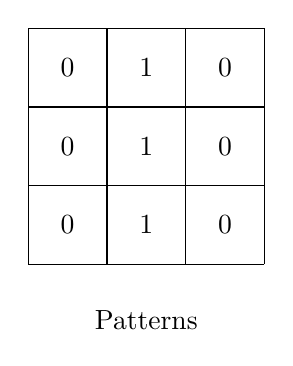
\begin{tikzpicture}
    \draw (0, 0) grid ++(3, 3);
    \foreach \i in {0, ..., 2} {
      \foreach \j in {0, ..., 2} {
        \ifnum\i=1
          \draw ({\i+0.5}, {\j+0.5}) node {1};
        \else
          \draw ({\i+0.5}, {\j+0.5}) node {0};
        \fi
      }
    }

      \draw (1.5, -0.7) node {Patterns};
      % 1. patterns
      % other things
  \end{tikzpicture}
\end{slide}

\begin{slide}{Convolutional Neural Networks: Intuition}
  \frameheader{What's in a kernel?}

  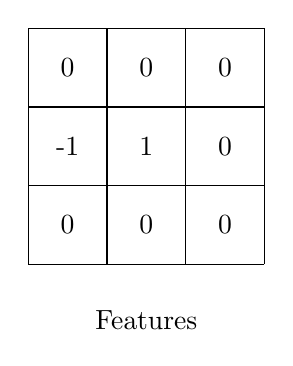
\begin{tikzpicture}
    \draw (0, 0) grid ++(3, 3);
    \foreach \i in {0, ..., 2} {
      \foreach \j in {0, ..., 2} {
        \ifnum\j=1
          \ifnum\i=0
            \draw ({\i+0.5}, {\j+0.5}) node {-1};
          \else
            \ifnum\i=1
              \draw ({\i+0.5}, {\j+0.5}) node {1};
            \else
              \draw ({\i+0.5}, {\j+0.5}) node {0};
            \fi
          \fi
        \else
          \draw ({\i+0.5}, {\j+0.5}) node {0};
        \fi
      }
    }

      % When the two pixels are similar, the two values cancel
      % When they are different (near edges), they give a large value
      \draw (1.5, -0.7) node {Features};
      % 1. patterns
      % other things
  \end{tikzpicture}
\end{slide}

\begin{slide}{Convolutional Neural Networks: Intuition}
  \includegraphics[scale=0.45]{weights}
\end{slide}
